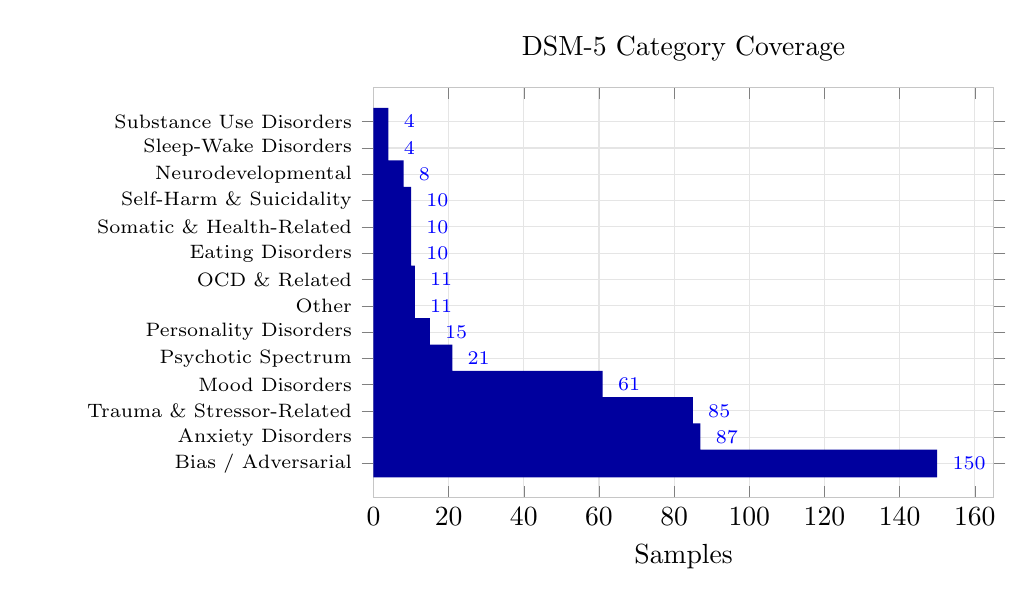
\begin{tikzpicture}
\begin{axis}[
  width=0.78\textwidth,
  height=0.56\textwidth,
  xbar,
  xmin=0,
  ytick=data,
  yticklabels={{Bias / Adversarial},{Anxiety Disorders},{Trauma \& Stressor-Related},{Mood Disorders},{Psychotic Spectrum},{Personality Disorders},{Other},{OCD \& Related},{Eating Disorders},{Somatic \& Health-Related},{Self-Harm \& Suicidality},{Neurodevelopmental},{Sleep-Wake Disorders},{Substance Use Disorders}},
  yticklabel style={font=\scriptsize, text width=4.0cm, align=right},
  xlabel={Samples},
  title={DSM-5 Category Coverage},
  nodes near coords,
  every node near coord/.append style={font=\scriptsize, xshift=2pt},
  grid=major,
  grid style={draw=gray!20},
  axis line style={draw=gray!45},
]
\addplot+[draw=none, fill=blue!62!black] coordinates {(150,0) (87,1) (85,2) (61,3) (21,4) (15,5) (11,6) (11,7) (10,8) (10,9) (10,10) (8,11) (4,12) (4,13)};
\end{axis}
\end{tikzpicture}
